%!TEX root =../../course-notes.tex
% ^ leave for LaTeXTools build functionality

\begin{applicationActivities}{3}{27}

\begin{observation}
Consider the linear transformation $A : \IR^2 \rightarrow \IR^2$ given by the matrix $A = \begin{bmatrix} 2 & 2 \\ 0 & 3 \end{bmatrix}$

\begin{center}
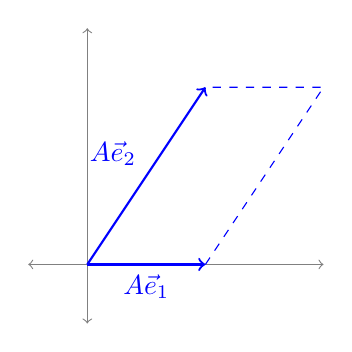
\begin{tikzpicture}[scale=0.75]
\draw[thin,gray,<->] (-1,0)-- (4,0);
\draw[thin,gray,<->] (0,-1)-- (0,4);
\draw[thick,blue,->] (0,0) -- node[below] {$A \vec{e}_1$}++ (2,0);
\draw[thick,blue,->] (0,0) -- node[above left] {$A \vec{e}_2$}++(2,3);
\draw[blue,dashed] (2,0) -- (4,3) -- (2,3);
\end{tikzpicture}
\end{center}
It is easy to see from the matrix $A$ that  $$A\vec{e_1} = A\begin{bmatrix}1 \\ 0 \end{bmatrix} = 2 \begin{bmatrix}1 \\ 0 \end{bmatrix} = 2 \vec{e_1}$$

It is less obvious (but easily verified) that
$$A\begin{bmatrix} 2 \\ 1 \end{bmatrix} = \begin{bmatrix} 6 \\ 3 \end{bmatrix} = 3\begin{bmatrix} 2 \\ 1 \end{bmatrix}$$
\end{observation}

\begin{definition}Let $A \in \IR^{n \times n}$.
An \term{eigenvector} is a vector $\vec{x} \in \IR^n$ such that $A\vec{x}$ is parallel to $\vec{x}$; in other words, $A\vec{x}=\lambda \vec{x}$ for some scalar $\lambda$, which is called an \term{eigenvalue}
\end{definition}

\begin{observation}
Observe that $A\vec{x}=\lambda \vec{x}$ is equivalent to $(A-\lambda I)\vec{x} = 0$.
\begin{itemize}
\item To find eigenvalues, we need to find values of $\lambda$ such that $A-\lambda I$ has a nontrivial kernel; equivalently, $A-\lambda I$ is not invertible, which is equivalent to $\det(A-\lambda I)=0$.  
\item $\det(A-\lambda I)$ is called the \term{characteristic polynomial} of $A$.  It is a polynomial in the variable $\lambda$.
\item Once an eigenvalue is found, the eigenvectors form a subspace called the \term{eigenspace}, which is simply the kernel of $A-\lambda I$.  Each eigenvalue will have an associated eigenspace.
\end{itemize}
\end{observation}

\begin{activity}{20}
Let $A = \begin{bmatrix} 2 & 2 \\ 0 & 3 \end{bmatrix}$.
\begin{subactivity}
Compute $\det \begin{bmatrix} 2-\lambda & 2 \\ 0 & 3-\lambda \end{bmatrix}$ to determine the characteristic polynomial of $A$.
\end{subactivity}
\begin{subactivity}
Find the roots of the characteristic polynomial to determine the eigenvalues of $A$.
\end{subactivity}
\begin{subactivity}
Compute the kernel of $A-2I$ to determine the eigenspace associated to the eigenvalue $3$.
\end{subactivity}
\begin{subactivity}
Compute the kernel of $A-3I$ to determine the eigenspace associated to the eigenvalue $3$.
\end{subactivity}
\end{activity}


\begin{activity}{15}
  Find all the eigenvalues and associated eigenspaces for the matrix $A=\begin{bmatrix} 3 & -2 & 1 \\  0 & 2 & 8 \\ 0 & 2 & 2 \end{bmatrix}$.

\begin{subactivity}
 Compute $\det (A-\lambda I)$ to determine the characteristic polynomial of $A$.
\end{subactivity}
\begin{subactivity}
Find the roots of the characteristic polynomial to determine the eigenvalues of $A$.
\end{subactivity}
\begin{subactivity}
Compute the kernel of $A-\lambda I$ for each eigenvalue $\lambda$ to determine the respective eigenspaces.
\end{subactivity}
\end{activity}

\begin{activity}{15}
  Find all the eigenvalues and associated eigenspaces for the matrix $A=\begin{bmatrix} 6 & -2 & 1 \\ 17 & -5 & 5 \\ -4 & 2 & 1 \end{bmatrix}$.

\begin{subactivity}
 Compute $\det (A-\lambda I)$ to determine the characteristic polynomial of $A$.
\end{subactivity}
\begin{subactivity}
Find the roots of the characteristic polynomial to determine the eigenvalues of $A$.
\end{subactivity}
\begin{subactivity}
Compute the kernel of $A-\lambda I$ for each eigenvalue $\lambda$ to determine the respective eigenspaces.
\end{subactivity}
\end{activity}

\end{applicationActivities}
